\section{Results}
\label{sec:results}

This section presents an evaluation of our JPEG-like compression system across multiple parameter sweeps and test scenarios. The goal is to assess compression performance with respect to visual quality, file size, semantic preservation, and runtime efficiency.

\subsection{Overview of Evaluation Goals}
Our evaluation focuses on the following:
\begin{itemize}
    \item \textbf{Visual Fidelity}: Comparison of output image quality under various compression settings
    \item \textbf{Compression Ratio}: Size reduction achieved with each configuration
    \item \textbf{Semantic Preservation}: Classification consistency of compressed images using pre-trained models
    \item \textbf{Runtime Performance}: Timing analysis for compression and decompression operations
\end{itemize}

\subsection{Test Methodology}
Experiments are conducted using YAML configurations across:
\begin{itemize}
    \item \texttt{compression\_configurations/\allowbreak quantization\_sweep/}
    \item \texttt{compression\_configurations/\allowbreak downsample\_sweep/}
    \item \texttt{compression\_configurations/\allowbreak block\_size\_sweep/}
    \item \texttt{compression\_configurations/\allowbreak quantization\_sweep\_chroma/}
    \item \texttt{compression\_configurations/\allowbreak quantization\_sweep\_luma/}
    \item \texttt{compression\_configurations/\allowbreak quantization\_sweep\_small\_blocks/}
\end{itemize}

Each configuration is tested on a standardized dataset of images (\texttt{assets/test\_images/}) with various formats and content types. Results are logged in corresponding metrics files (.metrics.json) and visual artifacts are stored in \texttt{results/}.

These additional sweeps were introduced after the initial draft to better isolate compression artifacts and parameter sensitivity across chroma and luma components.

To assist with analysis and visualization, we created a dedicated Jupyter notebook (\texttt{notebooks/plot\_results.ipynb}) to plot trends in PSNR, SSIM, compression ratios, and runtime performance across different sweep parameters.

\textit{Insert evaluation table or summary here when ready}

\subsection{Compression Quality}
% TODO: add PSNR/SSIM charts, or image quality metrics.
Placeholder: Figures will be added here comparing PSNR and/or SSIM across sweep configurations. Add compression ratio graphs (original vs compressed file size).

\subsection{Semantic Preservation}
Images were evaluated using a pre-trained classification model (e.g., ResNet50) to test whether compression degrades semantic content. This was done using \texttt{test/classification\_tests.py}.

\subsubsection{Semantic Preservation Metric}

Evaluating the Semantic Preservation of a compression algorithm is essentially asking \enquote Does the compressed image produce the same classification result with the same model input parameters? \enquote. A competing requirement for compression performance is compression ratio, or the fraction of image data the compressed encoded image takes up. As the compression ratio approaches zero, it's expected that the semantic content of the image would be lost. Therefore, understanding what compression parameters improve compression rate without degrading semantic content is the subject of exploration for this next section.

We propose Confidence Error as a general summary metric for Semantic Preservation. Let $C_{err}$ represent our metric, the Confidence Error. Let $L_{max}$ be the highest probability label from and inference pass with Resnet50 on the uncompressed image. Let $P^{Lmax}_{uncompressed}$ be the probability of this label. Let $P^{Lmax}_{compressed}$ be the classification probability of label $L_{max}$ on the compressed image.

$$
\textrm{C}_{err} = \frac{\|P^{Lmax}_{uncompressed} - P^{Lmax}_{compressed}\|}{P^{Lmax}_{uncompressed}}
$$

When performing parameter sweeps across various compression parameters, we evaluate Confidence Error with the following algorithm
\begin{algorithm}
    \label{alg:Confidence Error Algorithm}
    \caption{Evaluating Confidence Error during compression parameter sweeps}
    \textbf{Input: } Reference image $I_{ref}$, compressed image $I_{cmp}$, pretrained model $Res50$
    \textbf{Output: } $C_{err}$ for the two images
    \begin{itemize}
        \item $I_{ref, pp}$ = preprocess($I_{ref}$)
        \item $W_{ref outputs}$ = $Res50$.inference($I_{ref, pp}$)
        \item $P_{ref classes}$ = softmax($W_{outputs}$)
        \item $L_{max}$ = argmax({$P_{ref classes}$})
        \item $P^{Lmax}_{uncompressed}$ = $P_{classes}$[$L_{max}$]
        \item $I_{cmp, pp}$ = preprocess($I_{comp}$)
        \item $W_{comp outputs}$ = $Res50$.inference($I_{cmp, pp}$)
        \item $P_{cmp classes}$ = softmax($W_{outputs}$)
        \item $P^{Lmax}_{compressed}$ =  $P_{cmp classes}$[$L_{max}$]
        \item $\textbf{return}\ \frac{P^{Lmax}_{uncompressed} - P^{Lmax}_{compressed}}{P^{Lmax}_{uncompressed}}$
        \end{itemize}
    \end{algorithm}

%TODO: Add Description of preprocessing and classification for resnet50 to Implementation Section.

In this way, the semantic content is systematically compared and evaluated for each of the test images.

\subsubsection{Test Images}

In order to evaluate our compression pipeline, a set of test images with a variety of objects for classification was chosen. Resnet50 is a model largely for objects and non-human subjects, so images with a clear subject well centered in the image, spanning range of sizes relative to the size of the image. Additionally, some images were deliberately chosen because they contain multiple subjects or subjects where the classification is somewhat ambiguous, to see if these are more adversely effected by the compression than clear images. All test images are evaluated against all compression configurations. A set of novel images for classification are chosen for benchmarking rather than ImageNet or ResNet training set images to avoid compounding effects of muliple lossy compressions on the image. ImageNet and ResNet images are already JPEG images, and therefore have some (unknown) level of compression already applied to them. The test set images are either raw formats or lossless image formats (such as .png, and .webp).

% TODO: Incude table with the test images used for semantic preservation testing.

\subsubsection{JPEG Compression as a baseline for Semantic Preservation}

As a natural starting point of comparison for Semantic Preservation, we evaluate the semantic preservation of the JPEG compression standard.
The JPEG standard only exposes a single compression parameter available for adjustment, the JPEG Quality Factor (QF) largly effects the quantization table values for each of the Descrete-Cosine-Transformed Blocks.
Images are evaluated for semantic preservation using algorithm \ref{alg:Confidence Error Algorithm}.
Results are then parameterized by compression rate and original image content (figure \ref{fig:Comp vs Ratio JPEG Baseline}). There appears to be an inflection point around compression ratios of 0.1 or less, where certain images loose nearly all of their semantic content. For certain images, even ratios of 0.01 do not increase confidence error.

Taking a closer look at these images, images where the subject is large relative to the frame of the image have their semantic classifications more well preserved even with extremely agressive compression. However, When images contain other objects than the subject, or the subject of the image is small, the compression has a more dramatic impact on the classification. This trend is highlighted in figure \ref{fig:Annotated JPEG Baseline}

\begin{figure}
    \label{fig:Comp vs Ratio JPEG Baseline}
    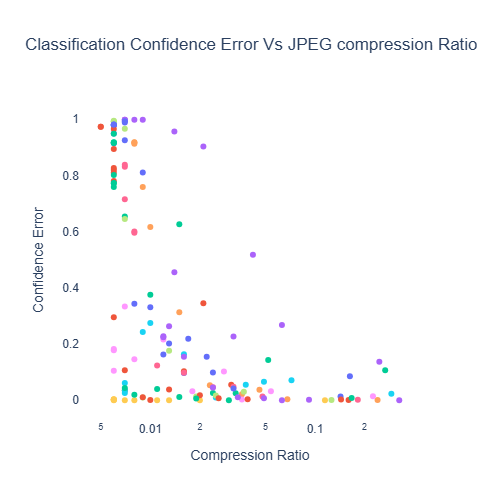
\includegraphics[width=0.5\textwidth]{assets/Baseline JPEG Confidence vs Comp Ratio.png}
    \caption{Confidence Error vs Compression Ratio for JPEG Compression. Smaller Values on the X axis correspond to smaller compressed images, while higher values on the Y axis correspond to a higher classification error rate. It appears that compression rates have little to no effect on semantic content until the compression ratio dips below 0.1.}
\end{figure}

\begin{figure}
    \label{fig:Annotated JPEG Baseline}
    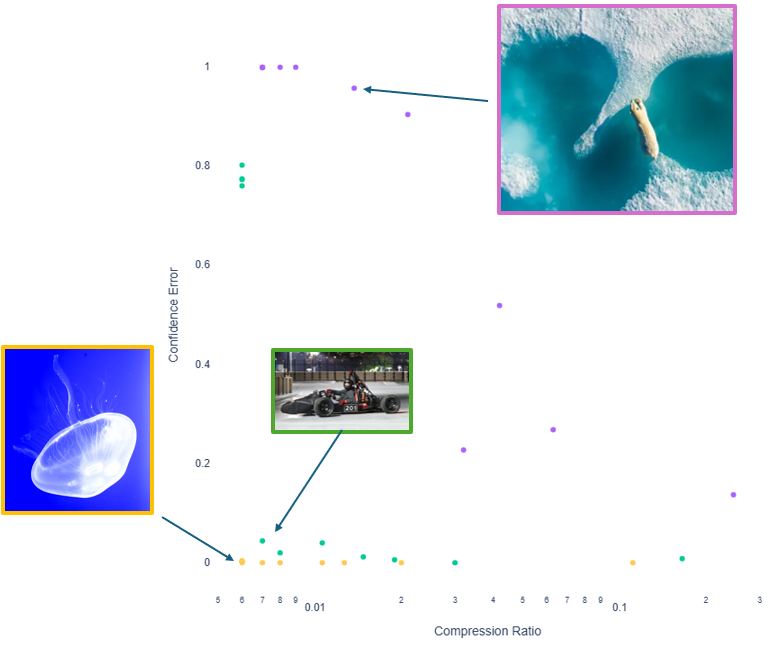
\includegraphics[width=0.5\textwidth]{assets/JPEG Baseline Compression with Examples}
    \caption{Certain Images have their semantic content preserved even with extremely agressive compression parameters where images are reduced to 0.6\% of their original size. Other images suffer from a sharp decline preserved semantic information. Intuitively, the higher the percentage of pixels in the image that represent the subject of classificatoin (as in the case of the jellyfish and the racecar), the better semantic preservation through compression.}
\end{figure}

The results for JPEG compression on these test images can serve as a baseline for other compression parameters evaluated.

\subsubsection{Quantization Sweep Results}

One of the compression parameters that our flexible compression pipeline makes available are the Quantization Tables.
These can be generated using Gaussian of the bottom right distance or scaled min and max values by the L-N Norm distances.
When Quantization is increased, more of the high-frequency information of the image is lost, so by sweeping through a set of quantization parameters, we can demonstrate the relative sensitivity of semantic information on high vs low frequency components.
The flexible compression pipeline also enables setting of luminance and chrominance quantization seperately, so we can explore whether semantic information is more closely tied to Luminance, or Chrominance information.

The parameters for Chrominance and Luminance quantization tested are listed in table \ref{tab:Quantization Parameters Table}. For sweeps with just Luminance or just Chrominance varried, the other quantization channel is processed with no Quantization.
All experiments use a Chrominance downsample factor of 2.

\begin{table}[h!]
\centering
\caption{Sample Table Caption}
\label{tab:Quantization Parameters Table}
\begin{tabular}{c|c|c|c|c}
\toprule
\textbf{Parameter Summary} & \textbf{Max Luma Quant} & \textbf{Luminance $\sigma$} & \textbf{Max Chroma Quant} & \textbf{Chrominance $\sigma$} \\
\midrule
No Quantization & 1 & 1 & 1 & 1 \\
High Quality & 10 & 3 & 20 & 3 \\
Quality & 30 & 5 & 40 & 5 \\
Moderate Quality & 60 & 6 & 75 & 6 \\
Low Quality & 100 & 8 & 125 & 8 \\
Very Low Quality & 150 & 10 & 200 & 10 \\
\bottomrule
\end{tabular}
\end{table}

Similar to the JPEG baseline, Confidence Error increases sharply when the compression rate drops below 0.1, as shown in figure \ref{fig:Confidence vs Quantization}
Interestingly however, when just the Chrominance or just the Luminance channels are varried, both the Confidence error and the compression ratio suffer. Shown in figure \ref{fig:just chroma or luma downsampling}

\begin{figure}
    \label{fig:Confidence vs Quantization}
    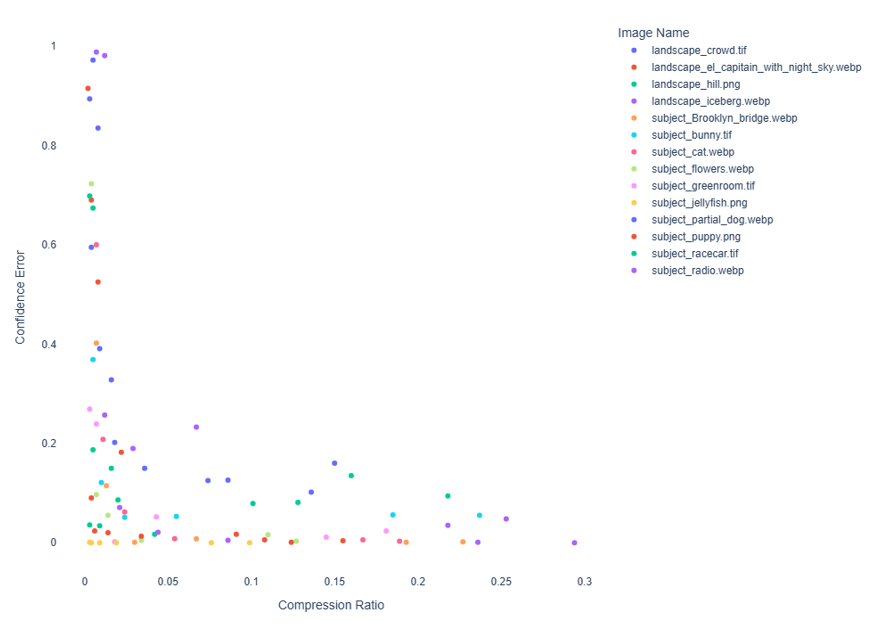
\includegraphics[width=0.5\textwidth]{assets/Quantization Sweep No Title Chrominance and Luminance.png}
    \caption{Confidence Error vs Compression Ratio as the Quantization parameters are varried. Quantization has very little effect on Semantic information until the compression ratio gets below approximately 0.1.}
\end{figure}
\begin{figure}
    \label{fig:just chroma or luma downsampling}
    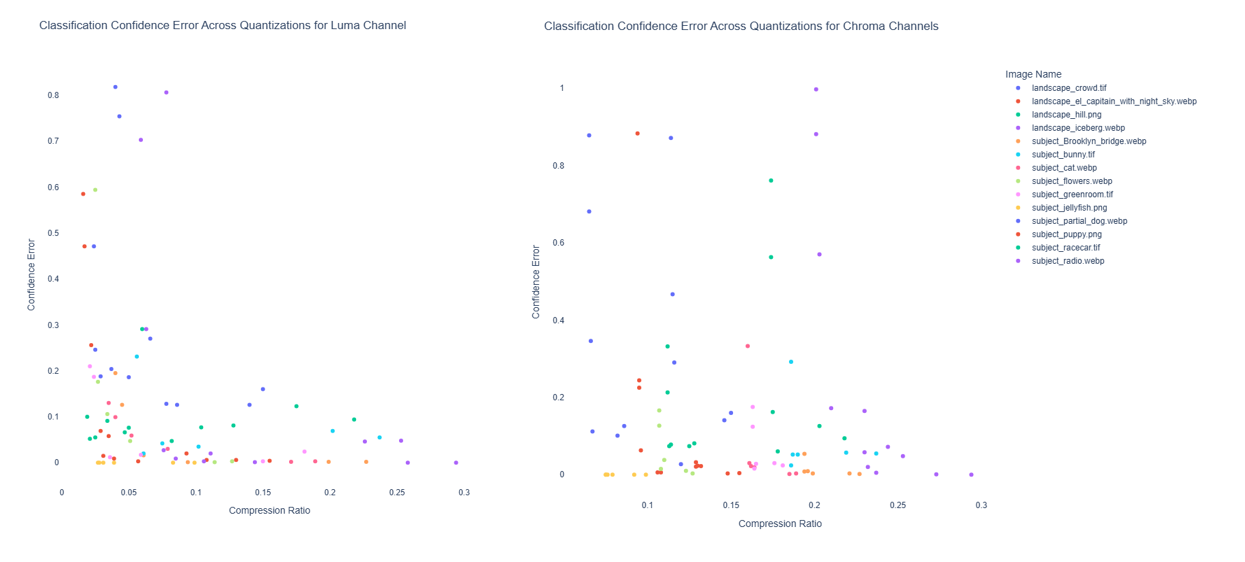
\includegraphics[width=0.5\textwidth]{assets/Chroma and Luma downsampling combined.png}
    \caption{Unlike in \ref{fig:Confidence vs Quantization}, if just one of the channel types is quantized, the semantic information is quickly lost, and the compression ratio is not improved.}
\end{figure}

\subsubsection{Block Size}

Block size affects the compressed result by changing pixel block base unit the Descrete Cosine Transform operates on.
Larger Blocks include a wider range of frequencies and more information being transformed each time, while smaller blocks allow for discontinuities at block edges to potentially go unnoticed.
In this experiment, we test apply our compression to images while varrying block size.

\begin{figure}
    \label{fig:block_size_sweep}
    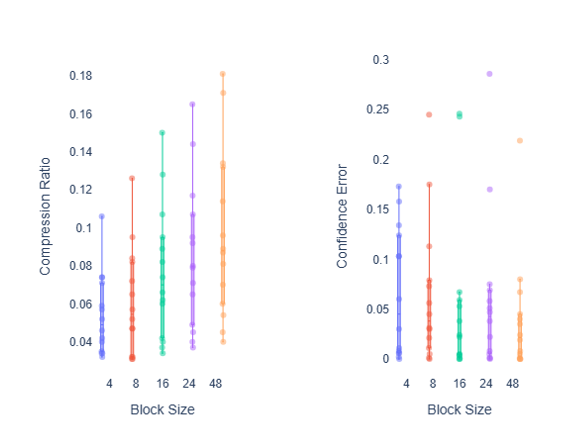
\includegraphics[width=0.5\textwidth]{assets/Confidence Err Vs Block Size.png}
    \caption{Confidence Error vs Compression Ratio for a variety of block sizes. The compression ratio }
\end{figure}
\subsection{Runtime and Performance}
% TODO: populate runtime benchmarks from .metrics.json
Execution time for both compression and decompression is measured and stored during sweeps. Aggregate runtime plots can be shown here.

\textit{Insert line/bar plots of compression vs. decompression runtime across settings}

\subsection{Discussion}
This subsection will summarize observed trends from the plots once all data is collected.

\textit{Pending: Discuss how image quality trades off with size reduction, runtime trends, and what configurations offered best balance}

% Note to team:
\textbf{NOTE TO TEAM:} Feel free to add figures using the `figure' environment, or tables using `table'. If any scripts output LaTeX-ready tables/plots, drop them in here. If results are still being generated, you can drop bullet points or markdown-style notes and we will convert them later.

\begin{itemize}
    \item \texttt{Use \textbackslash includegraphics\{filename\}} for figures stored in the same folder
    \item Comment clearly where plots/data are pending so we can track what still needs work
    \item Mention which script produced a plot to help trace reproducibility
\end{itemize}